%% LyX 2.0.5.1 created this file.  For more info, see http://www.lyx.org/.
%% Do not edit unless you really know what you are doing.
\documentclass[12pt]{report}
\usepackage{mathptmx}
\renewcommand{\familydefault}{\rmdefault}
\usepackage[T1]{fontenc}
\usepackage[latin9]{inputenc}
\usepackage[a4paper]{geometry}
\geometry{verbose,tmargin=2cm,bmargin=2cm,lmargin=2cm,rmargin=2cm,headheight=1cm,headsep=1cm,footskip=1cm}
\setcounter{secnumdepth}{2} % Changed from 3 to 2. 0-chapter 1-section 2-subsection 
\setcounter{tocdepth}{2} % Changed from 3 to 2. 0-chapter 1-section 2-subsection 
\setlength{\parskip}{\medskipamount}
\setlength{\parindent}{0pt}
\usepackage{verbatim}
\usepackage{pdfpages}
\usepackage{graphicx}
\usepackage{setspace}
\usepackage[numbers]{natbib}
\usepackage{nomencl}
% the following is useful when we have the old nomencl.sty package
\providecommand{\printnomenclature}{\printglossary}
\providecommand{\makenomenclature}{\makeglossary}
\makenomenclature
\doublespacing

\makeatletter

%%%%%%%%%%%%%%%%%%%%%%%%%%%%%% LyX specific LaTeX commands.
\providecommand{\LyX}{L\kern-.1667em\lower.25em\hbox{Y}\kern-.125emX\@}
%% Because html converters don't know tabularnewline
\providecommand{\tabularnewline}{\\}
%% A simple dot to overcome graphicx limitations
\newcommand{\lyxdot}{.}


%%%%%%%%%%%%%%%%%%%%%%%%%%%%%% User specified LaTeX commands.
\usepackage{tauthesis}
\usepackage[font={small,bf}, labelfont={small,bf}, margin=1cm]{caption}
\usepackage{titlesec}
\newcommand{\hsp}{\hspace{20pt}}
\titleformat{\chapter}[hang]{\Huge\bfseries}{\thechapter\hsp}{0pt}{\Huge\bfseries}


\Title{\textbf{Thesis Title}}
\Author{First Last}
\Year{August 2013}
\Supervisor{Prof. Alex Liberzon}
\Department{School of Mechanical Engineering}
\Degree{Master of Science}
% \Degree{Doctor of Philosophy}

\makeatother

\begin{document}
\begin{comment}
This is Micheal JasonSmith's uocthesis example ported to \LyX{} by
Etienne Lalibert� (etiennlaliberte@gmail.com).

Alex Liberzon (alex.liberzon@gmail.com) modified it to the Tel Aviv
University format, with the logo of the Faculty of Engineering. Change
the file taulogo.png to get the logo of your department.

Go to \textsf{Document > Settings > \LaTeX{} preamble} to modify the
\textsf{Title, Author, Year, Supervisor, Department} fields.

Default processor is now DVIPDFM - but if you can choose something
else, try PDFLATEX and XELATEX - sometimes these are a bit faster. 
\end{comment}


\prelimpages

\titlepage

\acknowledgments{I would like to thank my ...}

\begin{comment}
Split the thesis into separate chapters. Use \textbackslash{}include
mode to include the separate files.

Use \LyX{} Table of Contents, List of Figures, List of Tables and
Nomenclature automatics to include them in the thesis. Double - click
on each item to change the default level of contents, move the chapters
up/down and so on.
\end{comment}

\cleardoublepage
\setcounter{page}{1} % Start preliminary pages numbering (roman numerals).
%% LyX 2.0.5.1 created this file.  For more info, see http://www.lyx.org/.
%% Do not edit unless you really know what you are doing.

\chapter*{Abstract}

In this paper we investigate the issue of resource matching between jobs and machines in Intel's compute farm. We show that common heuristics such as Best-Fit and Worse-Fit may fail to properly utilize the available resources when applied to either cores or memory in isolation. In an attempt to overcome the problem we propose Mix-Fit, a heuristic which attempts to balance usage between resources. While this indeed usually improves upon the single-resource heuristics, it too fails to be optimal in all cases. As a solution we default to Max-Jobs, a meta-heuristic that employs all the other heuristics as sub-routines, and selects the one which matches the highest number of jobs. Extensive simulations that are based on real workload traces from four different Intel sites demonstrate that Max-Jobs is indeed the most robust heuristic for diverse workloads and system configurations, and provides up to 22% reduction in the average wait time of jobs.  


    

\tableofcontents{}

\listoffigures

\listoftables

\printnomenclature{}

\textpages


\chapter{Introduction}
%=====================

Intel owns an Internet-scale distributed compute farm that is used for
running its massive chip-simulation workloads
\citet[p.\ 78]{bentley01,evans03:book}.
The farm is composed of tens of thousands of servers that are located
in multiple data centers that are geographically spread around the
globe.
It is capable of running hundreds of thousands of simulation jobs and
tests simultaneously, and handles a rate of thousands of newly
incoming jobs every second.

This huge compute capacity is managed by an in-house developed
highly-scalable two-tier resource management and scheduling system
called \nb.
At the lower level \nb\ groups the servers into autonomous clusters
that are referred to in \nb\ terminology as Physical Pools.
Each such pool contains up to thousands of servers and is managed by a
single \nb\ entity that is called the Physical Pool Manager or PPM.
The role of the PPM is to accept jobs from the upper level, and to
schedule them on underlying servers efficiently and with minimal
waste.

At the upper level \nb\ deploys a second set of pools that are called
Virtual Pools.
Just like in the lower level, each virtual pool is managed by a single
\nb\ component that is called the Virtual Pool Manager or VPM.
The role of the VPMs is to cooperatively accept jobs from the users
and distribute them to the different PPMs in order to spread the load
across the farm.
Together, these two layers, VPMs at the top and PPMs at the
bottom, strive to utilize every compute resource across the farm.
This paper focuses on the work done at the PPM level.

A basic requirement in \nb\ is the enforcement of fair-share
scheduling among the various projects and business units within Intel
that share the farm.
Fair-share begins at the planning phase where different projects
purchase different amounts of servers to be used for their jobs.
These purchases eventually reflect their share of the combined
resources.
Once the shares are calculated, they are propagated to the PPMs where
they are physically enforced. (The calculation and propagation
mechanisms are beyond the scope of this paper.)

To enforce fair-share the PPM constantly monitors which jobs from
which projects are currently running and the amount of resources they
use.
The PPM then selects from its wait queue the first job from the most
eligible project (the project whose ratio of currently used resources
to its share of the resources is the smallest) and tries to match a
machine to that job.
If the matching succeeds, the job is scheduled for execution on that
machine.
Otherwise, a reservation is made for the job, and the process is
repeated while making sure not to violate previously made
reservations.
Such reservations enable jobs from projects that are lagging behind to
obtain the required resources as soon as possible.

Matching machines to jobs is done using any of a set of heuristics.
For example, one may sort the list of candidate machines according to
some pre-defined criteria --- e.g.\ increasing number of free cores or
decreasing amount of free memory --- and then traverse the sorted list
and select the first machine on which the job fits.
This leads to variants of \bef\ and \wof\ schemes.
Good sorting criteria reduce fragmentation thus allowing more jobs to be
executed, and are critical for the overall utilization of the pool.
Alternatively one may opt to reduce overhead and use a
\fif\ heuristic.

The sorting criteria are programmable configuration parameters in \nb.
This allows one to implement various matching heuristics and apply
them on different resources to best suit the workload characteristics
and needs.
\nb\ also allows individual jobs to specify different heuristics,
while the pool administrator can set a default policy to be used for
all jobs.

In this paper we argue that no heuristic applied to a
single resource in isolation can yield optimal performance under all
scenarios and cases.
To demonstrate our point we use both simple test cases and workload
traces that were collected at four large Intel sites.
Using the traces, we simulate the PPM behavior when applying the
different heuristics to schedule the jobs.
We show that depending on the workload different heuristics may be
capable of scheduling a higher number of jobs.

In an attempt to overcome the problem we develop ``\mif'' --- a
combined heuristic that tries to balance the use of cores and memory.
Intuitively this should reduce fragmentation at the pool.
However, while generally better than the previous heuristics,
\mif\ too fails to yield optimal assignments in some cases.

As an alternative, we propose a meta-heuristic we call ``\maj''.
\maj\ is not tailored towards specific workloads or configurations.
Instead, it uses the aforementioned heuristics as sub-routines and
chooses, in every scheduling cycle, the one that yields the highest
number of matched jobs.
This overcomes corner cases that hinder specific heuristics from being
optimal in all cases, and conforms well to the \nb\ philosophy of
maximizing resource utilization in every step.
We demonstrate, through simulation, that \maj\ yields lower wait times
by up to 22\% for all jobs in average under high loads.
%Interestingly, we also find that \mif\ produces scheduling decisions
%that are very close to those of \maj.

The rest of this paper is organized as follows.
Section \ref{sec:matching} provides more details on the problem of
matching machines to jobs, and explores the performance of commonly
used heuristics.
Section \ref{sec:mixed-fit} then describes the \mif\ heuristic,
followed by the \maj\ meta-heuristic in Section \ref{sec:max-jobs},
and simulation results in Section \ref{sec:sim_results}.
Section \ref{sec:related} briefly presents related work, and Section
\ref{sec:conclusions} concludes the paper.



\chapter{Matching Machines to Jobs}
%==================================
\label{sec:matching}

As described above, matching machines to jobs at the PPM is done by
choosing the most eligible job from the wait queue, sorting the list
of candidate machines according to some pre-defined criterion,
traversing the sorted list, and selecting the first machine on which
the job fits\footnote{This is done for practical reasons since trying
  all combinations is time consuming.}.
This is repeated again and again until either the wait queue or the
list of machines are exhausted.
At this point the PPM launches the chosen job(s) on the selected
machine(s) and waits for the next scheduling cycle.

A job may be multithreaded, but we assume that each job can fit on a
single (multicore) machine.
In principle \nb\ also supports parallel jobs (called ``MPI jobs'')
that span multiple machines, but in practice their numbers at the
present time are small.
The only added difficulty in supporting such jobs is the need to
allocate multiple machines at once instead of one at a time.

%Selecting the optimal match of jobs to machines is difficult problem that
%may be time consuming. Since scheduling cycles are short, and  \nb\
%strive to reduce the overhead of that calculation, a heuristic is employed
%to sort the machines. 
There are many criteria by which the machines can be sorted.
In this paper we focus on the number of free cores and amount of free
memory, as this suits well the workload in Intel which is
characterized by compute-intensive memory-demanding jobs.
Though I/O is definitely a factor, and some jobs do perform large file
operations, there are some in-house solutions that are beyond the
scope of this paper that greatly reduce the I/O burden on the
machines.

\begin{figure}[p]\centering
%	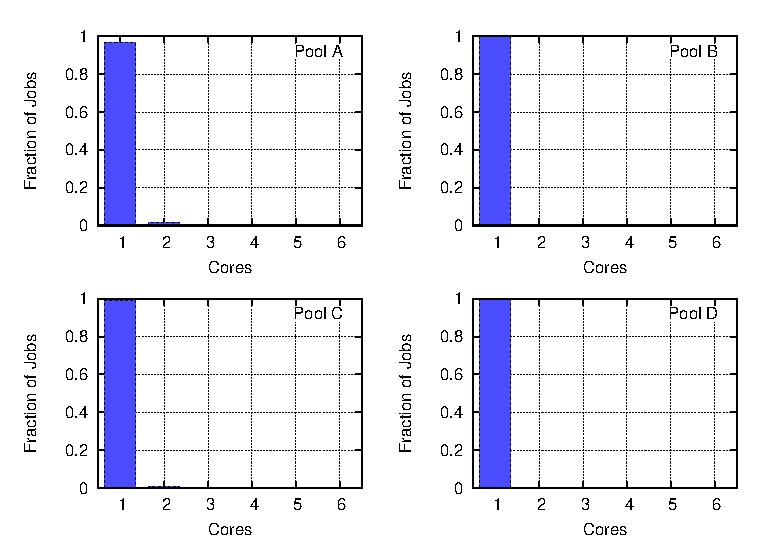
\includegraphics[width=.9\textwidth]{figures/cores_multiplot.eps}
	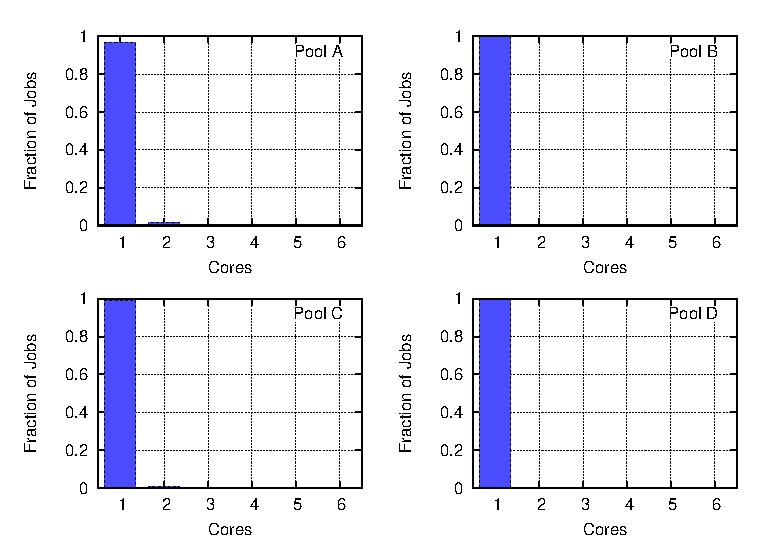
\includegraphics{figures/cores_multiplot.eps}
\caption{Jobs' cores requirements: the vast majority of the jobs are
  serial and require a single CPU core in order to execute.}
\label{fig:cores_usage_multiplot}
%\end{figure}
%\begin{figure}\centering
%	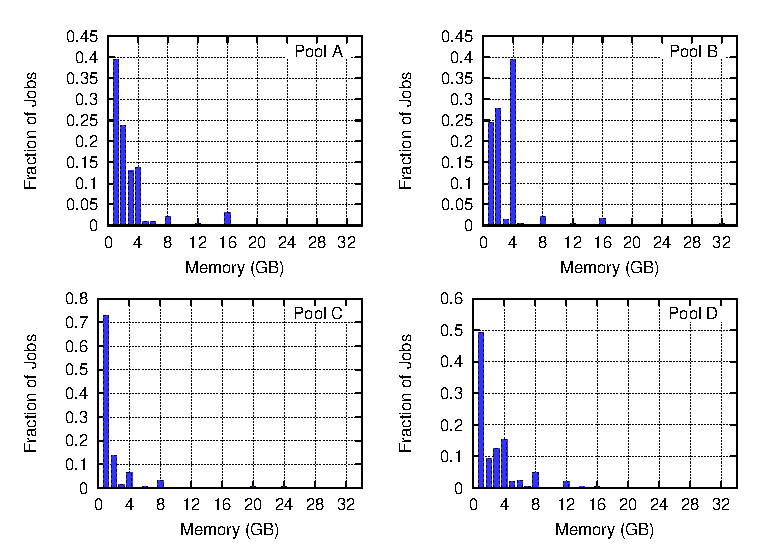
\includegraphics[width=1.0\textwidth]{figures/memory_multiplot.eps}
	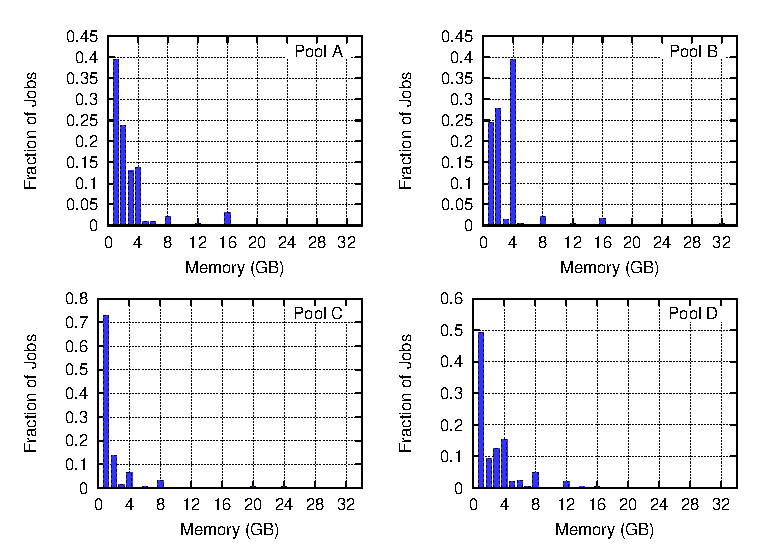
\includegraphics{figures/memory_multiplot.eps}
\caption{Jobs' memory requirements: demands are mostly 8 GB and below,
  but there are jobs that require 16 GB, 32 GB or even more memory in
  order to execute.}
\label{fig:memory_usage_multiplot}
\end{figure}

%At Intel, job is a process that is submitted with a definition of
%processors and memory requirements for its execution. Job can be parallel and
%require one or few cores, and a specific amount of memory in GB. 
Figures \ref{fig:cores_usage_multiplot} and \ref{fig:memory_usage_multiplot}
show the distribution of the jobs' cores and memory requirements in four large pools at different locations across the Intel farm%
\footnote{The requirements are specified as part of the job profile at submit time.}.
The data comes from traces \cite{parallel13} that were collected at the PPM
level during a one-month period, and which contain up to 13 million jobs each.
As can be seen in the figures, the vast majority of the jobs are
serial (single-thread jobs, requiring a single CPU core in order to execute).
Memory requirements are mostly 8 GB and below, but there are jobs that
require 16 GB, 32 GB, or even more memory (not shown) in order to
execute.
These observations are consistent across the pools.

%Figure \ref{fig:cores_mem_dist} shows the distribution of the jobs' cores and memory requirements in one of Intel's largest pools. The data comes from a trace that was collected during a one-month period and which contains more than 13 million jobs. As can be seen in Figure \ref{fig:cores_dist}, the vast majority of the jobs are serial and require a single CPU core in order to execute. Memory demands are mostly 8GB and below, but there are jobs that require 16GB, 32GB, or even more memory (not shown) in order to execute.

%\begin{figure}\centering
%\subfigure[\label{fig:cores_dist}Jobs' cores requirements]{
%	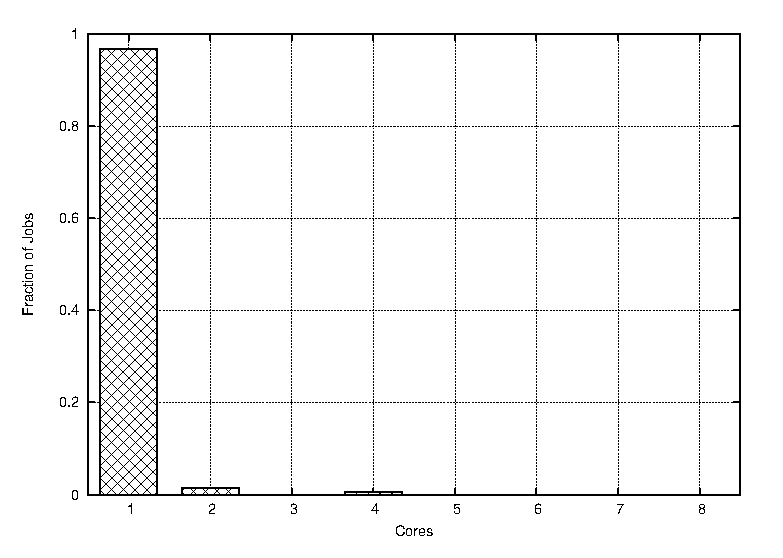
\includegraphics[width=0.45\textwidth]{figures/cores.eps}}
%\subfigure[\label{fig:mem_dist}Jobs' memory requirements]{
%	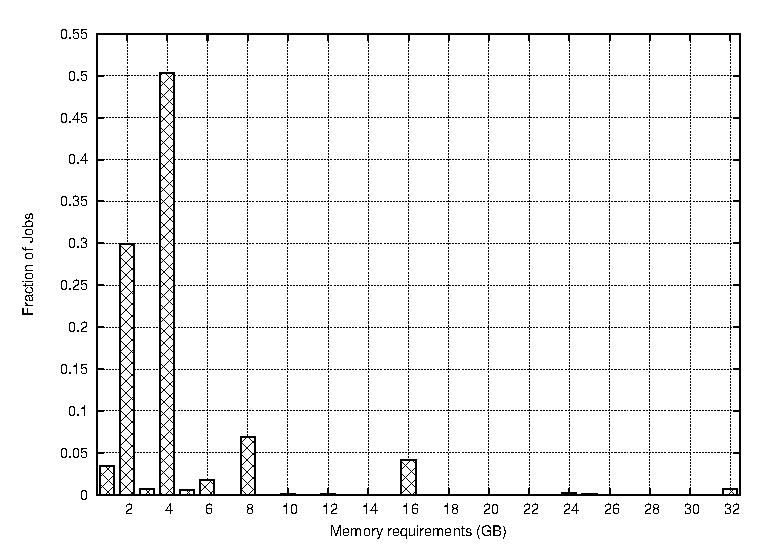
\includegraphics[width=0.45\textwidth]{figures/memory.eps}}
%\caption{Jobs' cores and memory requirements: (a) the vast majority of the jobs are serial and require a single CPU core in order to execute. (b) Memory demands are mostly 8GB and below, but there are jobs that require 16GB, 32GB or even more memory in order to execute.}
%\label{fig:cores_mem_dist}
%\end{figure}


The two ways to sort the machines by available cores or memory are in
increasing or decreasing order.
Sorting them by \textit{increasing} amount of free cores or memory and
selecting the first machine on which the job fits effectively
implements the \bef\ heuristic.
\bef\ is known to result in a better packing of jobs, while
maintaining unbalanced cores (or memory) usage across the machines in
anticipation for future jobs with high resource requirements.
Sorting the machines by \textit{decreasing} amount of free cores or
memory implements the \wof\ heuristic.
\wof's advantage is in keeping resource usage balanced across
machines, which is particularly useful for mostly-homogeneous
workloads.
For completeness we also mention \fif.
\fif's advantage is in its simplicity, as it does not require the
sorting of the machines.
Our tests, however, revealed that it performs poorly in our
environment, so we do not refer to it further in this paper.

We argue that no single heuristic, when applied to a single resource in
isolation, can yield optimal performance under all workload
scenarios.
To demonstrate our point we begin by providing simple synthetic examples
showing how different heuristics match different number of jobs under
different workload conditions.
We then put theory to the test by running simulations on the
aforementioned traces, demonstrating the effectiveness of the different heuristics 
under different workloads.


\section{Synthetic Examples of Heuristics Failures}
%-----------------------------------------------------

In our examples we consider two machines, A and B, each having four
cores and 32 GB of memory.
Assume that 8 jobs are queued at the PPM in the following priority order: two jobs
of one core and 16 GB of memory, and then 6 jobs of one core and 4 GB of
memory.
As can be seen in Figure \ref{fig:wf_better_A}, \bef\ matches the first
two jobs with machine A, totally exhausting its memory, and the next
four jobs with machine B, thereby exhausting its cores.
The end result is two unutilized cores on machine A, half the memory
unutilized on machine B, and two jobs that remain pending at the PPM.
\wof\ on the other hand matches the first two jobs on different
machines, which leaves enough free space (cores and memory) for all the
remaining 6 jobs to be matched.
This is illustrated in Figure \ref{fig:wf_better_B}.

\begin{figure}\centering
\subfigure[\label{fig:wf_better_A}\bef]{
	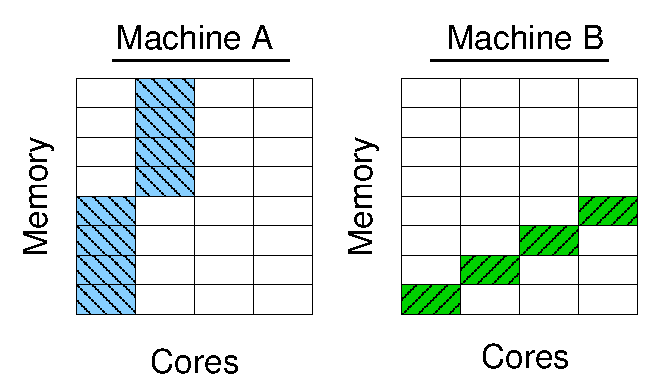
\includegraphics[width=0.45\textwidth]{figures/fig1a.eps}}
~~~~
\subfigure[\label{fig:wf_better_B}\wof]{
	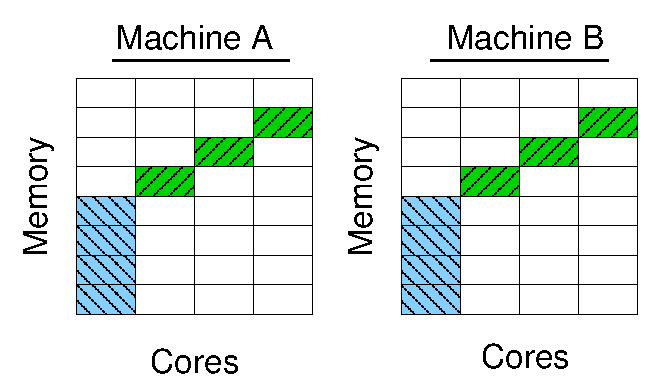
\includegraphics[width=0.45\textwidth]{figures/fig1b.eps}}
\caption{Scenario for which \wof\ (right) is better than \bef\ (left).
  Memory is depicted in 4 GB blocks.
  Shading indicates mapping of a job to a certain core and certain
  blocks of memory.
  Note that both cores and memory are mapped exclusively to distinct
  jobs.}
\label{fig:wf_better}
\end{figure}

Another example is illustrated in Figure \ref{fig:bf_better}.
The priority order here is 3 jobs of one core and 8 GB, followed by
one job of one core and 32 GB of memory.
As can be seen, \wof\ spreads the first three jobs on different
machines, which doesn't leaves enough memory for the 32 GB job to be
matched.
\bef\ on the other hand matches the first three jobs on machines A, 
which allows the 32 GB to be matched with machine B.

\begin{figure}\centering
\subfigure[\label{fig:bf_better_A}\bef]{
	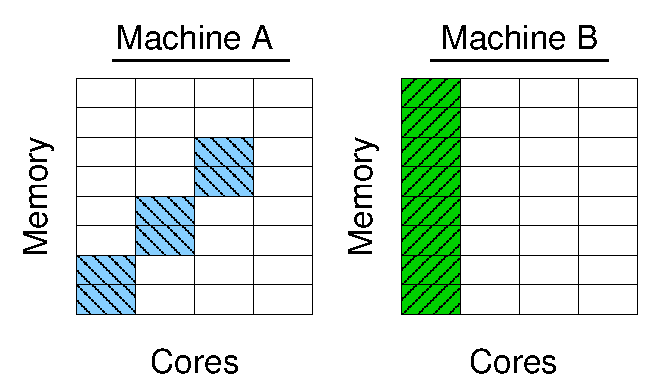
\includegraphics[width=0.45\textwidth]{figures/fig2b.eps}}
~~~~
\subfigure[\label{fig:bf_better_B}\wof]{
	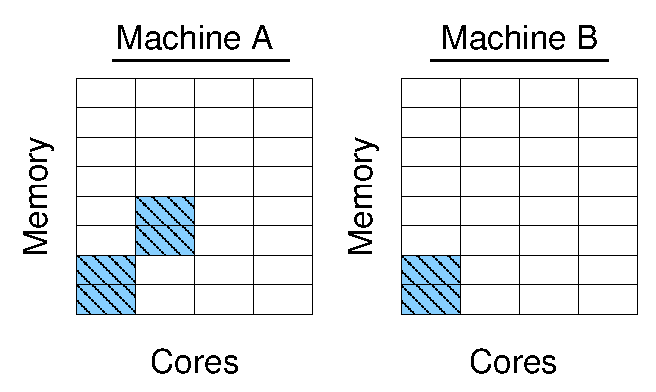
\includegraphics[width=0.45\textwidth]{figures/fig2a.eps}}
\caption{Scenario for which \bef\ (left) is better than \wof\ (right). }
\label{fig:bf_better}
\end{figure}





\bibliographystyle{plainnat}
\bibliography{references}

\appendix
\include{appendix}

\newpage{}

\begin{comment}
It is possible to create the Hebrew part in \LyX{}, but this is less
of our concern. Any typesetting software like \LyX{} (or Word or OpenOffice)
is as good for this purpose. After creating the PDF file from the
Hebrew document, include it here using the Insert -> File -> External
material -> PDFpages (one of the options). See the example below. 
\end{comment}


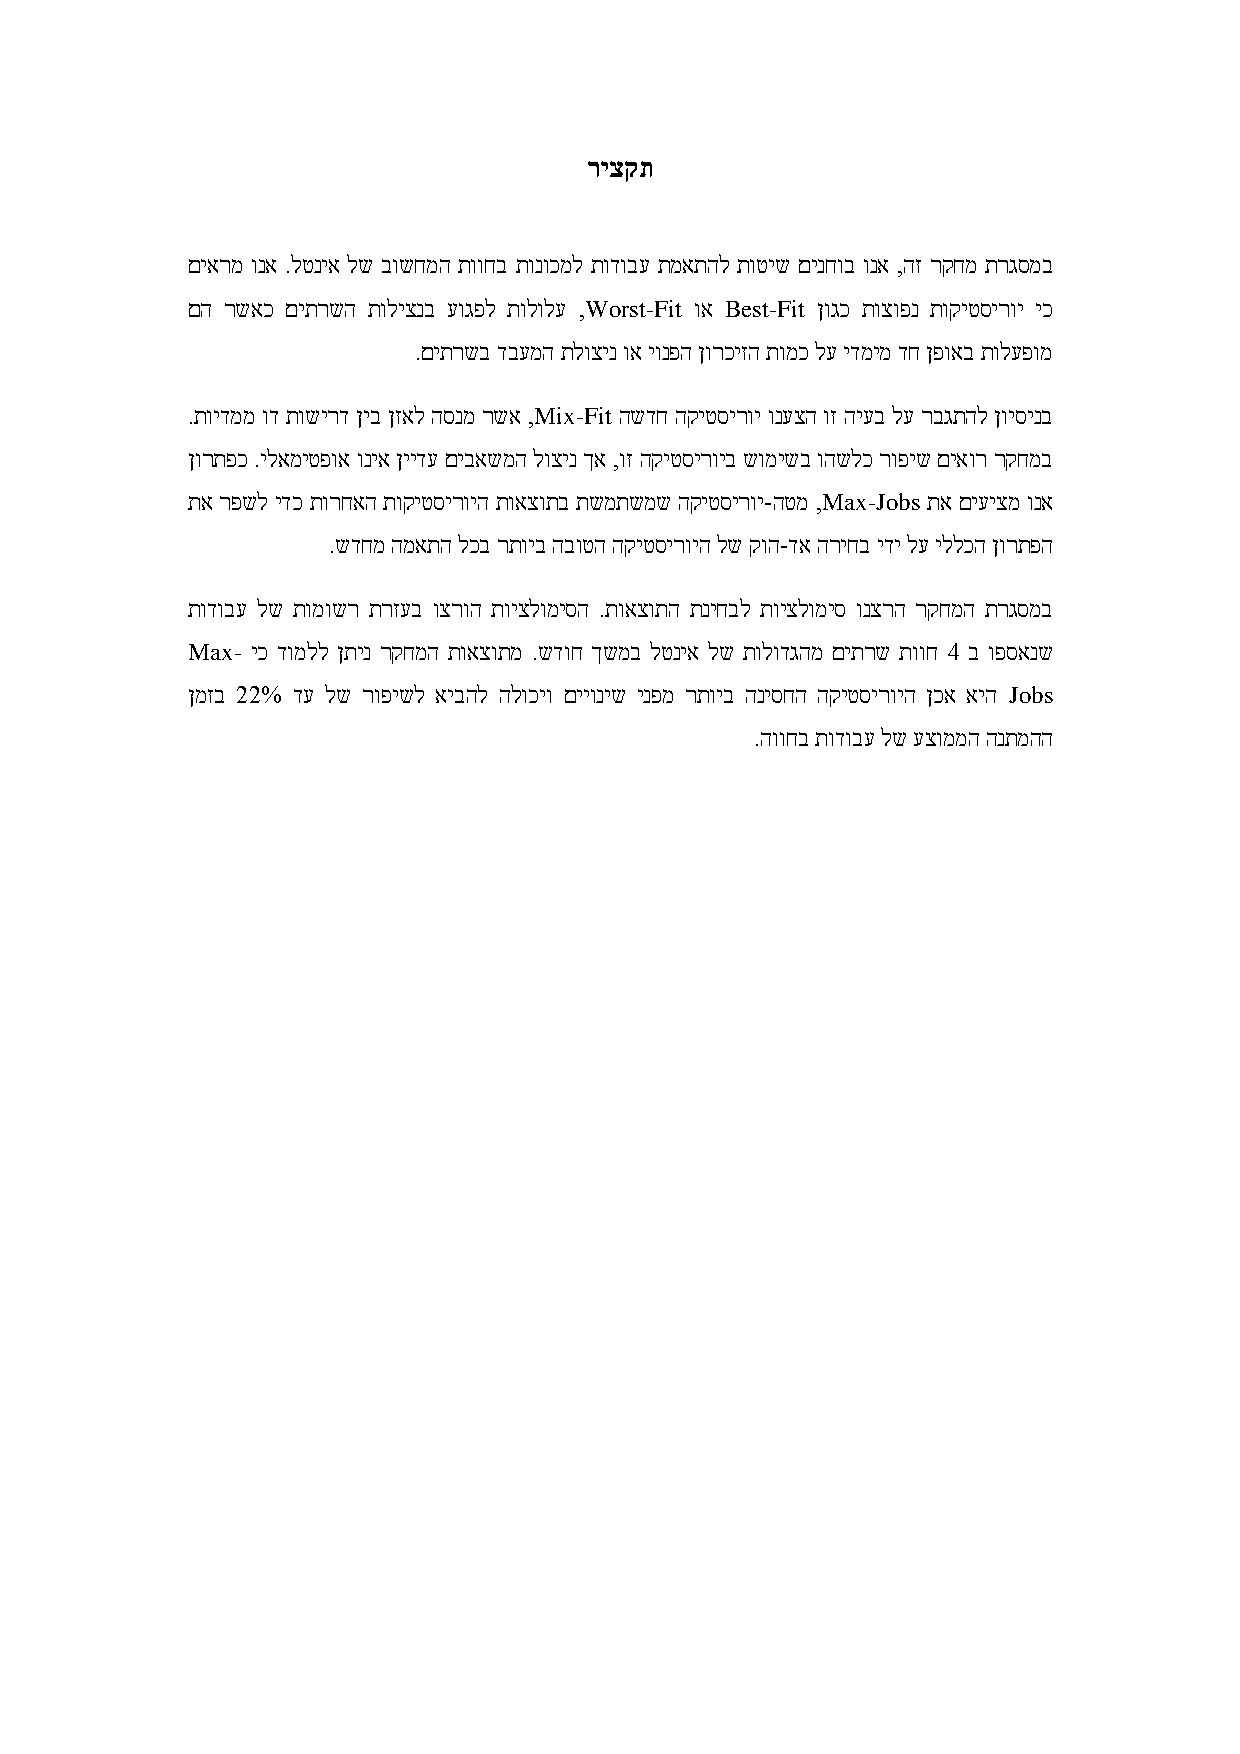
\includepdf[pages=-]{hebrew_part}
\end{document}
